
%Peter W.
%Requires the memoir class (as of this date v1.6180339e 2009/02/17)
%I suggest
\documentclass[oneside,11pt]{memoir}
%%% with the wide textblock, 12pt is too small for reading ease, so best not
%%% to use 11pt or 10pt.

%%% Arial
%\usepackage[T1]{fontenc}
%\usepackage[scaled]{uarial}
%\renewcommand*\familydefault{\sfdefault} %% Only if the base font of the document is to be sans serif

%%% Garamond
%\usepackage[T1]{fontenc}
%\usepackage{lmodern}
%\usepackage{garamond}

%%% MS San Serif
%\usepackage[T1]{fontenc}
%\usepackage[scaled]{helvet}
%\renewcommand*\familydefault{\sfdefault} %% Only if the base font of the document is to be sans serif

%%% Times
\usepackage{mathptmx}  % Times New Roman, but if you have Garamond then use it;
                       % you are writing a book, not a newspaper column
\DoubleSpacing         % memoir's double spacing
\usepackage{pwasu}     % this package

%%%%%%Added by Craig Picone to meet ASU's margin requirements
\usepackage{graphicx}    % needed for including graphics e.g. EPS, PS
\topmargin -0.2in        % read Lamport p.163
\oddsidemargin 0.5in   % read Lamport p.163
\evensidemargin 0in  % same as oddsidemargin but for left-hand pages
\textwidth 5.5in
\textheight 8.83in 
%\pagestyle{empty}       % Uncomment if don't want page numbers
\parskip 7.2pt           % sets spacing between paragraphs
%\renewcommand{\baselinestretch}{1.5} % Uncomment for 1.5 spacing between lines
\parindent 0pt          % sets leading space for paragraphs
 %%%%%%%%

%    The general sequence in your document, after you have set the data for
%the TITLE and APPROVAL pages, and any other specifics in the preamble is:
\DoubleSpacing
\begin{document}
\maxtocdepth{subparagraph} % put everything into the ToC
\pagestyle{plain}  % pagestyle for the prelims
\frontmatter
\thetitlepage
%%\approvalpage

%% Added by bbailey1
% Macro for List of Symbols
\def\listofsymbols{%%%%%%%%%%%%%%%%%%%%%%%
%Sample List of Symbols
%%%%%%%%%%%%%%%%%%%%%%%
\begin{tabbing}
% YOU NEED TO ADD THE FIRST ONE MANUALLY TO ADJUST THE TABBING AND SPACES
$n$~~~~~\=\parbox{5in}{Vector size\dotfill \pageref{symbol:nml}}\\
%ADD THE REST OF SYMBOLS WITH THE HELP OF MACRO
\addsymbol m: {Vector size}{symbol:nml}
\addsymbol l: {Vector size}{symbol:nml}
\addsymbol x: {State vector}{symbol:x}
\addsymbol u: {Control input}{symbol:x}
\addsymbol y: {Output vector}{symbol:x}
% .
% .
% .
\addsymbol \mathbf{A}: {State Matrix}{symbol:A}
\addsymbol \mathbf{B}: {Input Matrix}{symbol:B}
\addsymbol \mathbf{C}: {Output Matrix}{symbol:C}
% .
% .
% .
% ALWAYS KEEP THE FOLLOWING LINE
\end{tabbing} \clearpage}
\def\addsymbol #1: #2#3{$#1$ \> \parbox{5.45in}{#2 \dotfill \pageref{#3}}\\}
\def\newnot#1{\label{#1}}
 
 
%%%%%%%%%%%%%%%%%%%%%%%%%%%%%%%%%%%%%%%%%%%%%%%%%%%%%%%%%%%%%%%%%%%
% here is the main part of your dessertation
 
% put your abstract here
 
\asuabstract 
\setlength{\parindent}{.5in}
This is a sample abstract
 
% your acknowledgement

\setdedication{ Your dedication goes here. } % if you want a dedication
 
\asudedication

\asuacknowledgements
[Enter your text here]

\tableofcontents
\listoftables   % if you have any tables

\listoffigures  % if you have any figures

%% Added by bbailey1
%% Uncomment the next 3 lines for List of Symbols
% \newpage
% \chapter*{List of Symbols\hfill} \addcontentsline{toc}{chapter}{LIST OF SYMBOLS}
% \listofsymbols

%%
% Mark your variables in your source code with \newnot{YOUR_SYMBOL_LABEL}.
% Example:
% ...Here, if the dimensions of A \newnot{sybmol:A}, B \newnot{symbol:B}, and C \newnot{symbol:C} are
% nxn, nxm and lxn \newnot{symbol:nml} respectfully; then ...
%%

%\newpage
%\chapter*{PREFACE\hfill} \addcontentsline{toc}{chapter}{PREFACE}
%[Enter your text here]
%\clearpage

%% if you have more prelim sections, then
%%%\clearpage
%%%%%\pagestyle{plain}
%%%%%\prelimtitle   text % for sections after the ToC, etc, before main text
\mainmatter
\pagestyle{asu}

\addcontentsline{toc}{chapter}{CHAPTER}

\pagestyle{plain} 
% finally, start of your main text

\chapter{INTRODUCTION} 

\DoubleSpacing
\setlength{\parindent}{.5in}
Human interpersonal interactions are socially driven exchanges of verbal and non-verbal communicative cues. The essence of humans as social animals is very well exemplified in the way humans interact face-to-face with one another. Even in a brief exchange of eye gaze, humans communicate a lot of information about themselves, while assessing a lot about others around them. Though not much is spoken, plenty is always said. We still do not understand the nature of human communication and why face-to-face interactions are so significant for us. 

Social interaction refers to any form of mutual communication between two individuals or between an individual and a group \cite{riggio_assessment_1986}. Such communications involve any or all forms of sensory and motor activities as deemed necessary by the participants of the interaction. Social, Behavioral and Developmental Sociologists emphasize that the ability of individuals to effectively control expressive behavior is essential for the social and interpersonal functioning of our society. Such social interactions are the aggregate cause of social behaviors, social actions and social contact that helps not only in effective bilateral communication, but also in forming an efficient feedback driven behavioral learning loop. It is this feedback (termed as social feedback) that children use towards developing good social and communicative skills. 

Recent studies in behavioral psychology are furthering our understanding of the importance of social behaviors and social actions in everyday context. Researchers have revealed an unconscious need in humans to mimic and imitate the mannerisms of their interaction partners. An increasing number of experiments have highlighted this need for imitation to be very primeval and that they offer an elegant channel for building trust and confidence between individuals.

\section{Components of Social Interactions}
From a neurological perspective, social interactions result from the complex interplay of cognition, action and perception tasks within the human brain. For example, the simple act of shaking hands involves interactions of sensory, motor and cognitive events. Two individuals who engage in the act of shaking hands have to first make eye contact, exchange emotional desire to interact (this usually happens through a complex set of face and body gestures, such as smile and increased upper body movements), determine the exact distance between themselves, move appropriately towards each other maintaining Proxemics (interpersonal distance) that are befitting of their cultural setting, engage in shaking hands, and finally, move apart assuming a conversational distance which is invariably wider than the hand shake distance. Verbal exchanges may occur before, during or after the hand shake itself. This example shows the need for sensory (visual senses of face and bodily actions, auditory verbal exchange etc.), perceptual (understanding expressions, distance between individuals etc.), and cognitive (recognizing the desire to interact, engaging in verbal communication etc.) exchange during social interactions. Further, though social interactions display such complex interplay, they have been studied in the human communication literature under two important categories \cite{brent_d._ruben_human_1975}, namely, 

\begin{itemize}
\item \emph {Verbal communication}: Explicit communication through the use of words in the form of speech or transcript.
\item \emph {Non-verbal communication}: Implicit communication cues that use prosody, body kinesis, facial movements and spatial location to communicate information that may be unique or overlapping with verbal information. 
\end{itemize}

While the spoken language plays an important role in communiction, speech accounts for only 35\% of the interpersonal exchanges. Nearly 65\% of all information communication happens through non-verbal cues \cite{knapp_nonverbal_1996}. Out of this large chunk, 48\% of the communication, is through visual encoding of face and body kinesis and posture, while the rest is encoded in the prosody (intonation, pitch, pace and loudness of voice) \cite{borkenau_thin_2004}. A closer look at the various non-verbal communication modes can highlight the importance of the multimodality of social exchanges.

\subsection{Non-verbal communication cues}
Speech, voice, face and body form the primary channels of communication in any social interaction. Speech forms the primary channel for verbal communication, while prosody (intonation, pace and loudness of one’s voice), face, and body (posture, gesture and mannerisms) form the medium for nonverbal communication. In everyday social interactions, people communicate so effortlessly through both verbal and non-verbal cues that they are not cognizant of the complex interplay of their voice, face and body in establishing a smooth communication channel. 

\subsubsection{Social Sight and Social Hearing}
Unlike speech, which is mostly under the conscious control of the user, the non-verbal communication channels are engaged from a subconscious level. Though people can increase their control on these channels through training, innately, individuals demonstrate certain inability to control their non-verbal cues. This inability to control non-verbal channels is referred to as the leakiness \cite{brown_social_1986} and humans (evolutionarily) have learnt to pick up these leaked signals during social interactions. For example, people can read very subtle body mannerisms very easily to determine the mental state of their interaction partner. Eye Gaze is a classic example of such subtle cues where interaction partners can detect interest, focus, involvement and role play, to name a few.  On this leakiness scale, it has been found that the voice is the leakiest of all channels, implying that emotions of individuals are revealed first in their voice before any of the other channels are engaged. The voice is followed by body, face and finally the verbal channel, speech. The leakiness is plotted on the abscissa of Figure \ref{Figure1} with the ordinate showing the amount of information encoded in the other three non-verbal communication channels. It can be seen that the face communicates the most amount of non-verbal cues, while the prosody (voice) is the first channel to leak emotional information.

\begin{figure}
\begin{center}
 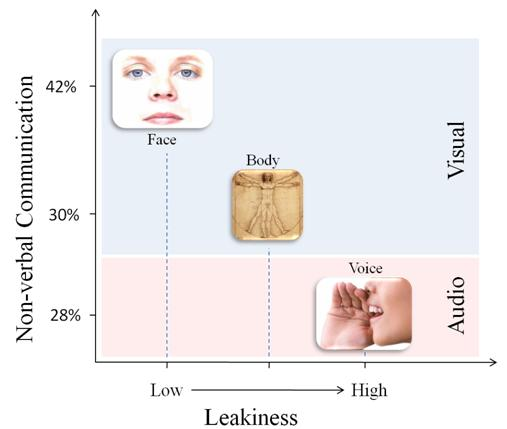
\includegraphics[width=4in]{Leakiness.jpg}
\caption{Relative communicative information plotted aganist its leakiness. Speech forms the verbal channel. Face, body and voice form the non-verbal communication channels.}
\end{center}
\label{Figure1}
\end{figure}

\subsubsection{Social touch}
Apart from visual and auditory channels of social stimulation, humans increasingly rely on social touch during interpersonal interactions. For example, hand shake represents an important aspect of social communication conveying confidence, trust, dominance and other important personal and professional skills \cite{burgoon_relational_1984}. Social touch has also been studied by psychologists in the context of emotional gratification. Wetzel \cite{wetzel_midas_1984} demonstrated patron gratification effects through tipping behavior when waitresses touched their patrons. Similar studies have revealed the importance of social touch and how conscious decision making is connected deeply with the human affect system. In the recent years social touch has gained a lot of interest in the area remote interactions \cite{haans_mediated_2006} \cite{bailenson_virtual_2008} to help better understand the nature of social situational awareness in social presence. 

\subsection{Decoding of non-verbal communication cues}

-----------------------------------------------
Inability or difficulty to access any part of this non-verbal cues, seriously affects the overall understanding of the social scene and reduces the involvement of an individual in the social interactions.
---------------------------------------------


\chapter{RELATED WORK} 

\DoubleSpacing
\setlength{\parindent}{.5in}
[Enter your text here]

\section{Test 1}
\subsection{Test 2}
\subsubsection{Test 3}

\clearpage


%\newpage
%\chapter*{REFERENCES\hfill} \addcontentsline{toc}{chapter}{REFERENCES}
\begin{SingleSpace}
\bibliographystyle{ieeetr}	
\bibliography{references}
\end{SingleSpace}
%\clearpage
 
%% maybe endnotes 
%% maybe bibliography
% if appendices, then

\appendix
\addcontentsline{toc}{chapter}{APPENDIX}
\chapter{\uppercase{Insert Appendix A Title here}}
\clearpage
\chapter{\uppercase{Insert Appendix B Title here}}
\clearpage

% if Biographical sketch then
%\newpage
%\newpage
%\begin{center}\bibname\end{center} \addcontentsline{toc}{chapter}{\bibname}
%\clearpage
%[Enter your text here]
%\clearpage
%\newpage	
This LaTeX document was generated using the Graduate College Format Advising tool. Please turn a copy of this page in when you submit your document to Graduate College format advising. You may discard this page once you have printed your final document. DO NOT TURN THIS PAGE IN WITH YOUR FINAL DOCUMENT! 


\end{document}		
		